\documentclass{article}
\usepackage[margin=0.75in]{geometry}
\usepackage{xcolor}
\usepackage{amsmath}
\usepackage{amssymb}
\usepackage{fontspec}
\usepackage{tikz}
\usetikzlibrary{tikzmark, arrows.meta, positioning, decorations.pathreplacing}
\usepackage{enumitem}
\usepackage{multicol}

% ---- Theme Colors ----
\definecolor{bglight}{HTML}{FFFFFF}
\definecolor{textlight}{HTML}{000000}
\definecolor{subtext}{HTML}{666666}

% ---- Bar Model Visual Colors ----
\colorlet{redbar}{red!70!black}
\colorlet{bluebar}{blue!55!black}
\colorlet{greenbar}{green!60!black}
\colorlet{yellowbar}{yellow!80!black}
\colorlet{arrowblue}{cyan!70!blue}

\pagecolor{bglight}
\color{textlight}

\pagestyle{empty}

% Numbered node macro from your theme
\newcommand{\stepnum}[2]{%
  \tikzmarknode{#2}{%
    \begin{tikzpicture}[baseline=(char.base)]
      \node[draw=textlight, circle, inner sep=1.5pt, font=\sffamily\small] (char) {#1};
    \end{tikzpicture}%
  }%
}

\begin{document}
\sffamily

% ================= HEADER =================
\begin{center}
  {\Huge \bfseries Bar Method Exercise Sheet} \\[0.4em]
  {\Large \textbf{Part-Whole Model}}
\end{center}
\vspace{1em}

\section*{Part 1: Visualizing Addition}

% ================= EXAMPLE SECTION =================
{\Large \textbf{Example: Finding Total Pencils}}
\vspace{0.3em}

\noindent Maya has \textbf{5 red pencils} and \textbf{3 blue pencils}. How many pencils does she have in total?
\vspace{0.8em}

\begin{description}[leftmargin=2em]

  \item[\stepnum{1}{s1}] \textbf{Identify and label the parts}\\[0.2em]
  Determine the quantities given in the problem:
  \begin{itemize}
    \item Red pencils = $5$
    \item Blue pencils = $3$
  \end{itemize}
  \vspace{0.6em}

  \item[\stepnum{2}{s2}] \textbf{Draw bars representing each part}\\[0.4em]
  Draw connected blocks proportional to each value to visualize the whole:
  \\[0.6em]
  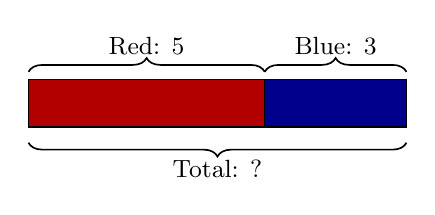
\begin{tikzpicture}[>=Stealth, baseline={(0,1.2)}]
    % Top brackets with labels
    \draw[decorate, decoration={brace, amplitude=5pt}, line width=0.6pt] (0, 1.8) -- (3, 1.8);
    \node[anchor=south] at (1.5, 1.9) {\small Red: 5};

    \draw[decorate, decoration={brace, amplitude=5pt}, line width=0.6pt] (3, 1.8) -- (4.8, 1.8);
    \node[anchor=south] at (3.9, 1.9) {\small Blue: 3};

    % Bars
    \draw[fill=redbar, draw=black, line width=0.5pt] (0, 1.1) rectangle (3, 1.7);
    \draw[fill=bluebar, draw=black, line width=0.5pt] (3, 1.1) rectangle (4.8, 1.7);

    % Bottom bracket for total
    \draw[decorate, decoration={brace, amplitude=5pt, mirror}, line width=0.6pt] (0, 0.9) -- (4.8, 0.9);
    \node[anchor=north] at (2.4, 0.8) {\small Total: ?};
  \end{tikzpicture}
  \vspace{0.6em}

  \item[\stepnum{3}{s3}] \textbf{Write and solve the equation}\\[0.4em]
  Combine the parts to calculate the overall total:
  \[
    5 + 3 = \mathbf{8} \quad \text{or} \quad 3 + 5 = \mathbf{8}
  \]
  \vspace{0.2em}
  Maya has \textbf{8 pencils} altogether.

\end{description}

\begin{tikzpicture}[remember picture, overlay]
  \draw[dotted, thick, textlight!60] (s1.south) -- (s2.north);
  \draw[dotted, thick, textlight!60] (s2.south) -- (s3.north);
\end{tikzpicture}

\vspace{1em}
\noindent\textcolor{subtext!40}{\rule{\linewidth}{0.5pt}}
\vspace{1.5em}

% ================= PRACTICE QUESTIONS =================
\begingroup
\parindent=0pt

{\Large \textbf{Practice Questions}}\par\vspace{0.4em}
Read each problem, fill in the missing numbers in the bar model, and solve.

\endgroup
\vspace{1.5em}

\begin{enumerate}[label=\textbf{\arabic*.}, itemsep=2.5em, leftmargin=2em]

  % Question 1
  \item \textbf{Lucas saved \$45 in January and \$38 in February. How much money did he save in total?}

  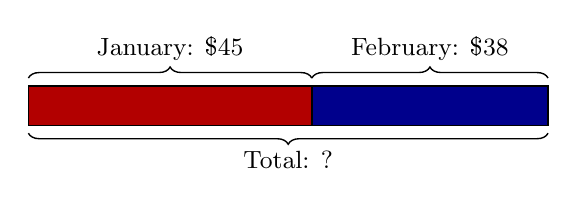
\begin{tikzpicture}[>=Stealth, baseline={(0,0.5)}]
    % Top brackets & Labels
    \draw[decorate, decoration={brace, amplitude=4pt}, line width=0.5pt] (0, 1.2) -- (3.6, 1.2);
    \node[anchor=south] at (1.8, 1.3) {\small January: \$45};

    \draw[decorate, decoration={brace, amplitude=4pt}, line width=0.5pt] (3.6, 1.2) -- (6.6, 1.2);
    \node[anchor=south] at (5.1, 1.3) {\small February: \$38};

    % Colored Bars
    \draw[fill=redbar, draw=black, line width=0.5pt] (0, 0.6) rectangle (3.6, 1.1);
    \draw[fill=bluebar, draw=black, line width=0.5pt] (3.6, 0.6) rectangle (6.6, 1.1);

    % Total Bracket
    \draw[decorate, decoration={brace, amplitude=4pt, mirror}, line width=0.5pt] (0, 0.5) -- (6.6, 0.5);
    \node[anchor=north] at (3.3, 0.4) {\small Total: ?};
  \end{tikzpicture}

  \vspace{0.5em}
  Equation: $\underline{\hspace{1.5cm}} + \underline{\hspace{1.5cm}} = \underline{\hspace{1.5cm}}$
  \hspace{2cm} Total savings = \$\underline{\hspace{1.5cm}}

  \clearpage

  % Question 2
  \item \textbf{John the baker made 240 cupcakes.}
  \begin{enumerate}[label=(\alph*)]
    \item \textbf{150 cupcakes were sold in the morning. How many cupcakes were left?}
    \item \textbf{If 80 cupcakes were sold in the afternoon, how many cupcakes does he have now?}
  \end{enumerate}

  \vspace{1em}

  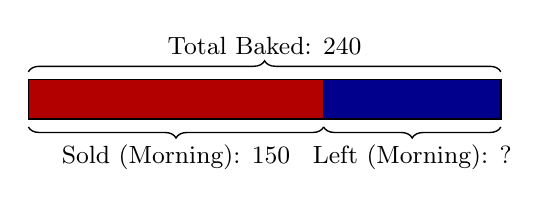
\begin{tikzpicture}[>=Stealth, baseline={(0,0.5)}]
    % Total Bracket on Top
    \draw[decorate, decoration={brace, amplitude=4pt}, line width=0.5pt] (0, 1.2) -- (6.0, 1.2);
    \node[anchor=south] at (3.0, 1.3) {\small Total Baked: 240};

    % Colored Bars
    \draw[fill=redbar, draw=black, line width=0.5pt] (0, 0.6) rectangle (3.75, 1.1);
    \draw[fill=bluebar, draw=black, line width=0.5pt] (3.75, 0.6) rectangle (6.0, 1.1);

    % Bottom Brackets
    \draw[decorate, decoration={brace, amplitude=4pt, mirror}, line width=0.5pt] (0, 0.5) -- (3.75, 0.5);
    \node[anchor=north] at (1.875, 0.4) {\small Sold (Morning): 150};

    \draw[decorate, decoration={brace, amplitude=4pt, mirror}, line width=0.5pt] (3.75, 0.5) -- (6.0, 0.5);
    \node[anchor=north] at (4.875, 0.4) {\small Left (Morning): ?};
  \end{tikzpicture}

  \vspace{0.6em}
  (a) Equation: $\underline{\hspace{1.5cm}} - \underline{\hspace{1.5cm}} = \underline{\hspace{1.5cm}}$
  \hspace{1cm} Cupcakes left = $\underline{\hspace{1.5cm}}$

  \vspace{1em}

    % Single combined bar model for total cupcakes (240) split into Morning, Afternoon, and Left
  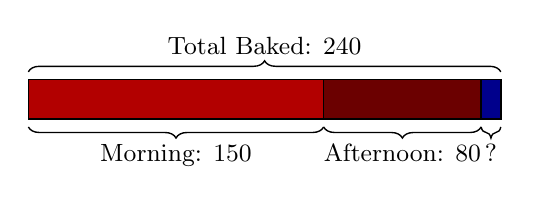
\begin{tikzpicture}[>=Stealth, baseline={(0,0.5)}]
    % Top Bracket for Overall Total
    \draw[decorate, decoration={brace, amplitude=4pt}, line width=0.5pt] (0, 1.2) -- (6.0, 1.2);
    \node[anchor=south] at (3.0, 1.3) {\small Total Baked: 240};

    % Colored Bars representing three parts of the whole
    \draw[fill=redbar, draw=black, line width=0.5pt] (0, 0.6) rectangle (3.75, 1.1);
    \draw[fill=redbar!60!black, draw=black, line width=0.5pt] (3.75, 0.6) rectangle (5.75, 1.1);
    \draw[fill=bluebar, draw=black, line width=0.5pt] (5.75, 0.6) rectangle (6.0, 1.1);

    % Bottom Brackets for each component
    \draw[decorate, decoration={brace, amplitude=4pt, mirror}, line width=0.5pt] (0, 0.5) -- (3.75, 0.5);
    \node[anchor=north] at (1.875, 0.4) {\small Morning: 150};

    \draw[decorate, decoration={brace, amplitude=4pt, mirror}, line width=0.5pt] (3.75, 0.5) -- (5.75, 0.5);
    \node[anchor=north] at (4.75, 0.4) {\small Afternoon: 80};

    \draw[decorate, decoration={brace, amplitude=4pt, mirror}, line width=0.5pt] (5.75, 0.5) -- (6.0, 0.5);
    \node[anchor=north] at (5.875, 0.4) {\small ?};
  \end{tikzpicture}

  \vspace{0.6em}
  
  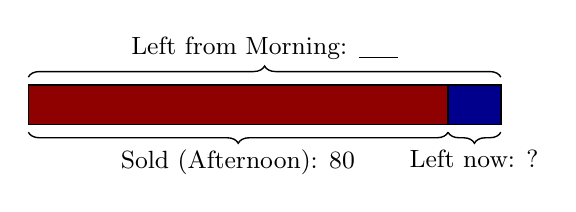
\begin{tikzpicture}[>=Stealth, baseline={(0,0.5)}]
    % Top Bracket showing remaining cupcakes from morning (90)
    \draw[decorate, decoration={brace, amplitude=4pt}, line width=0.5pt] (0, 1.2) -- (6.0, 1.2);
    \node[anchor=south] at (3.0, 1.3) {\small Left from Morning: \underline{\hspace{0.5cm}}};

    % Colored Bars dividing the remaining into sold afternoon vs final left
    \draw[fill=redbar!80!black, draw=black, line width=0.5pt] (0, 0.6) rectangle (5.33, 1.1);
    \draw[fill=bluebar, draw=black, line width=0.5pt] (5.33, 0.6) rectangle (6.0, 1.1);

    % Bottom Brackets
    \draw[decorate, decoration={brace, amplitude=4pt, mirror}, line width=0.5pt] (0, 0.5) -- (5.33, 0.5);
    \node[anchor=north] at (2.66, 0.4) {\small Sold (Afternoon): 80};

    \draw[decorate, decoration={brace, amplitude=4pt, mirror}, line width=0.5pt] (5.33, 0.5) -- (6.0, 0.5);
    \node[anchor=north] at (5.66, 0.4) {\small Left now: ?};
  \end{tikzpicture}

  \vspace{0.6em}
  (b) Equation: $\underline{\hspace{1.5cm}} - \underline{\hspace{1.5cm}} = \underline{\hspace{1.5cm}}$
  \hspace{1cm} Cupcakes left = $\underline{\hspace{1.5cm}}$

  % Question 3
  \item \textbf{Maya read $\frac{3}{8}$ of a book on Saturday and $\frac{2}{8}$ of it on Sunday. What fraction of the book does she have left to read?}

  \vspace{0.5em}
  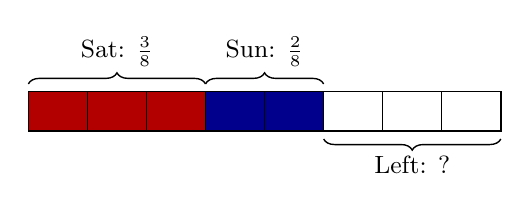
\begin{tikzpicture}[>=Stealth, baseline={(0,0.5)}]
    % Bar divided into 8 equal parts
    \draw[fill=redbar, draw=black, line width=0.5pt] (0, 0.6) rectangle (2.25, 1.1);
    \draw[fill=bluebar, draw=black, line width=0.5pt] (2.25, 0.6) rectangle (3.75, 1.1);
    \draw[fill=white, draw=black, line width=0.5pt] (3.75, 0.6) rectangle (6.0, 1.1);

    % Grid lines inside
    \foreach \x in {0.75, 1.5, 3.0, 4.5, 5.25} {
      \draw[line width=0.5pt] (\x, 0.6) -- (\x, 1.1);
    }

    % Top brackets
    \draw[decorate, decoration={brace, amplitude=4pt}, line width=0.5pt] (0, 1.2) -- (2.25, 1.2);
    \node[anchor=south] at (1.125, 1.3) {\small Sat: $\frac{3}{8}$};

    \draw[decorate, decoration={brace, amplitude=4pt}, line width=0.5pt] (2.25, 1.2) -- (3.75, 1.2);
    \node[anchor=south] at (3.0, 1.3) {\small Sun: $\frac{2}{8}$};

    % Bottom bracket
    \draw[decorate, decoration={brace, amplitude=4pt, mirror}, line width=0.5pt] (3.75, 0.5) -- (6.0, 0.5);
    \node[anchor=north] at (4.875, 0.4) {\small Left: ?};
  \end{tikzpicture}

  \vspace{0.6em}
  Fraction read = $\underline{\hspace{1.2cm}} + \underline{\hspace{1.2cm}} = \underline{\hspace{1.2cm}}$
  \hspace{1.5cm} Fraction left = $1 - \underline{\hspace{1.2cm}} = \underline{\hspace{1.2cm}}$

  % Question 4
  \item \textbf{A toy store has 520 red, blue, and green balls. 185 are red and 210 are blue. How many green balls are there?}

  \vspace{0.5em}
  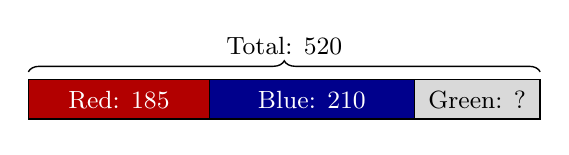
\begin{tikzpicture}[>=Stealth, baseline={(0,0.5)}]
    % Top Bracket Total
    \draw[decorate, decoration={brace, amplitude=4pt}, line width=0.5pt] (0, 1.2) -- (6.5, 1.2);
    \node[anchor=south] at (3.25, 1.3) {\small Total: 520};

    % Bars
    \draw[fill=redbar, draw=black, line width=0.5pt] (0, 0.6) rectangle (2.3, 1.1);
    \draw[fill=bluebar, draw=black, line width=0.5pt] (2.3, 0.6) rectangle (4.9, 1.1);
    \draw[fill=gray!30, draw=black, line width=0.5pt] (4.9, 0.6) rectangle (6.5, 1.1);

    % Labels inside or below
    \node at (1.15, 0.85) {\small\color{white}Red: 185};
    \node at (3.6, 0.85) {\small\color{white}Blue: 210};
    \node at (5.7, 0.85) {\small Green: ?};
  \end{tikzpicture}

  \vspace{0.6em}
  Green balls: $520 - 185 - 210 = \underline{\hspace{1.5cm}}$
  % \hspace{2cm} Green balls = $\underline{\hspace{1.5cm}}$

  % Question 5
  \item \textbf{A ribbon is 4.5 meters long. Hannah cuts off a piece measuring 1.85 meters. How long is the remaining ribbon?}

  \vspace{0.5em}
  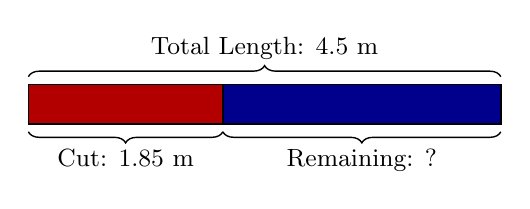
\begin{tikzpicture}[>=Stealth, baseline={(0,0.5)}]
    % Top Bracket Total
    \draw[decorate, decoration={brace, amplitude=4pt}, line width=0.5pt] (0, 1.2) -- (6.0, 1.2);
    \node[anchor=south] at (3.0, 1.3) {\small Total Length: 4.5 m};

    % Bars
    \draw[fill=redbar, draw=black, line width=0.5pt] (0, 0.6) rectangle (2.47, 1.1);
    \draw[fill=bluebar, draw=black, line width=0.5pt] (2.47, 0.6) rectangle (6.0, 1.1);

    % Bottom Brackets
    \draw[decorate, decoration={brace, amplitude=4pt, mirror}, line width=0.5pt] (0, 0.5) -- (2.47, 0.5);
    \node[anchor=north] at (1.235, 0.4) {\small Cut: 1.85 m};

    \draw[decorate, decoration={brace, amplitude=4pt, mirror}, line width=0.5pt] (2.47, 0.5) -- (6.0, 0.5);
    \node[anchor=north] at (4.235, 0.4) {\small Remaining: ?};
  \end{tikzpicture}

  \vspace{0.6em}
  Equation: $\underline{\hspace{1.5cm}} - \underline{\hspace{1.5cm}} = \underline{\hspace{1.5cm}}$ m
  \hspace{1.5cm} Remaining ribbon = $\underline{\hspace{1.5cm}}$ m

\end{enumerate}

  \clearpage

% ================= PART 2: COMPARISON MODELS =================
\section*{Part 2: Comparison Models (Two or More Quantities)}

\begin{enumerate}[label=\textbf{\arabic*.}, start=6, itemsep=2.5em, leftmargin=2em]

  \vspace{1em}
  % Question 6
  \item \textbf{Liam has 84 stamps. He has 26 more stamps than Noah. How many stamps does Noah have?}

  \vspace{0.5em}
  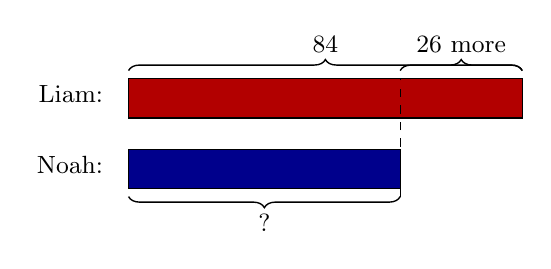
\begin{tikzpicture}[>=Stealth, baseline={(0,0.5)}]
    \node[anchor=east] at (-0.2, 1.2) {\small Liam:};
    \draw[fill=redbar, draw=black, line width=0.5pt] (0, 0.9) rectangle (5.0, 1.4);
    \draw[decorate, decoration={brace, amplitude=4pt}, line width=0.5pt] (0, 1.5) -- (5.0, 1.5);
    \node[anchor=south] at (2.5, 1.6) {\small 84};

    \node[anchor=east] at (-0.2, 0.3) {\small Noah:};
    \draw[fill=bluebar, draw=black, line width=0.5pt] (0, 0.0) rectangle (3.45, 0.5);
    \draw[decorate, decoration={brace, amplitude=4pt, mirror}, line width=0.5pt] (0, -0.1) -- (3.45, -0.1);
    \node[anchor=north] at (1.725, -0.2) {\small ?};

    \draw[dashed, line width=0.5pt] (3.45, -0.1) -- (3.45, 1.4);
    \draw[decorate, decoration={brace, amplitude=4pt}, line width=0.5pt] (3.45, 1.5) -- (5.0, 1.5);
    \node[anchor=south] at (4.225, 1.6) {\small 26 more};
  \end{tikzpicture}

  \vspace{0.6em}
  Equation: $\underline{\hspace{1.5cm}} - \underline{\hspace{1.5cm}} = \underline{\hspace{1.5cm}}$
  \hspace{2cm} Noah's stamps = $\underline{\hspace{1.5cm}}$

  \vspace{1em}

  % Question 7
  \item \textbf{Box A weighs 12 kg. Box B is 4 kg heavier than Box A. Box C is 3 kg lighter than Box B. What is the total weight of all three boxes?}

  \vspace{0.5em}
  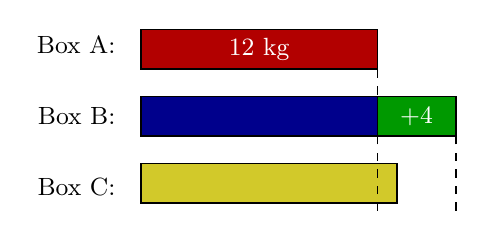
\begin{tikzpicture}[>=Stealth, baseline={(0,0.5)}]
    \node[anchor=east] at (-0.2, 1.8) {\small Box A:};
    \draw[fill=redbar, draw=black, line width=0.5pt] (0, 1.5) rectangle (3.0, 2.0);
    \node at (1.5, 1.75) {\small\color{white}12 kg};

    \node[anchor=east] at (-0.2, 0.9) {\small Box B:};
    \draw[fill=bluebar, draw=black, line width=0.5pt] (0, 0.65) rectangle (3.0, 1.15);
    \draw[fill=greenbar, draw=black, line width=0.5pt] (3.0, 0.65) rectangle (4.0, 1.15);
    \node at (3.5, 0.9) {\small\color{white}+4};

    \node[anchor=east] at (-0.2, 0.0) {\small Box C:};
    \draw[fill=yellowbar, draw=black, line width=0.5pt] (0, -0.2) rectangle (3.25, 0.3);

    \draw[dashed, line width=0.5pt] (3.0, -0.3) -- (3.0, 2.0);
    \draw[dashed, line width=0.5pt] (4.0, -0.3) -- (4.0, 1.15);
  \end{tikzpicture}

  \vspace{0.6em}
  Box B weight = $\underline{\hspace{1.2cm}} + \underline{\hspace{1.2cm}} = \underline{\hspace{1.2cm}}$ kg
  \hspace{1cm} Box C weight = $\underline{\hspace{1.2cm}} - \underline{\hspace{1.2cm}} = \underline{\hspace{1.2cm}}$ kg \\
  Total weight = $\underline{\hspace{1.2cm}} + \underline{\hspace{1.2cm}} + \underline{\hspace{1.2cm}} = \underline{\hspace{1.5cm}}$ kg

  \vspace{1em}

  % Question 8
  \item \textbf{Emma, Chloe, and Grace collected 360 seashells. Emma collected 40 more seashells than Chloe, and Grace collected twice as many seashells as Chloe. How many seashells did Chloe collect?}

  \vspace{0.5em}
  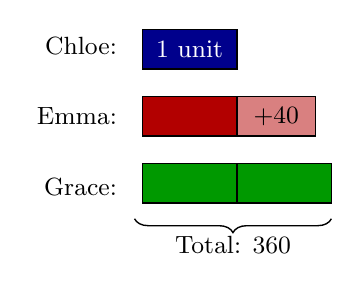
\begin{tikzpicture}[>=Stealth, baseline={(0,0.5)}]
    \node[anchor=east] at (-0.2, 1.8) {\small Chloe:};
    \draw[fill=bluebar, draw=black, line width=0.5pt] (0, 1.5) rectangle (1.2, 2.0);
    \node at (0.6, 1.75) {\small\color{white}1 unit};

    \node[anchor=east] at (-0.2, 0.9) {\small Emma:};
    \draw[fill=redbar, draw=black, line width=0.5pt] (0, 0.65) rectangle (1.2, 1.15);
    \draw[fill=redbar!50, draw=black, line width=0.5pt] (1.2, 0.65) rectangle (2.2, 1.15);
    \node at (1.7, 0.9) {\small +40};

    \node[anchor=east] at (-0.2, 0.0) {\small Grace:};
    \draw[fill=greenbar, draw=black, line width=0.5pt] (0, -0.2) rectangle (1.2, 0.3);
    \draw[fill=greenbar, draw=black, line width=0.5pt] (1.2, -0.2) rectangle (2.4, 0.3);

    \draw[decorate, decoration={brace, amplitude=5pt, mirror}, line width=0.5pt] (-0.1, -0.4) -- (2.4, -0.4);
    \node[anchor=north] at (1.15, -0.5) {\small Total: 360};
  \end{tikzpicture}

  \vspace{0.6em}
  $4 \text{ units} + 40 = 360 \implies 4 \text{ units} = \underline{\hspace{1.5cm}} \implies 1 \text{ unit} = \underline{\hspace{1.5cm}}$ \\
  Chloe collected = $\underline{\hspace{1.5cm}}$ seashells

  \clearpage

  % Question 9
  \item \textbf{The ratio of the number of apples to oranges in a basket is $4 : 7$. If there are 28 apples, how many oranges are there?}

  \vspace{0.5em}
  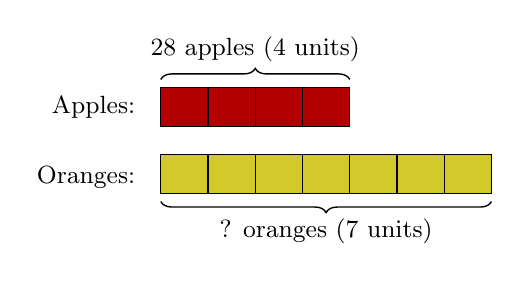
\begin{tikzpicture}[>=Stealth, baseline={(0,0.5)}]
    \node[anchor=east] at (-0.2, 0.9) {\small Apples:};
    \draw[fill=redbar, draw=black, line width=0.5pt] (0, 0.65) rectangle (2.4, 1.15);
    \foreach \x in {0.6, 1.2, 1.8} { \draw[line width=0.5pt] (\x, 0.65) -- (\x, 1.15); }
    \draw[decorate, decoration={brace, amplitude=4pt}, line width=0.5pt] (0, 1.25) -- (2.4, 1.25);
    \node[anchor=south] at (1.2, 1.35) {\small 28 apples (4 units)};

    \node[anchor=east] at (-0.2, 0.0) {\small Oranges:};
    \draw[fill=yellowbar, draw=black, line width=0.5pt] (0, -0.2) rectangle (4.2, 0.3);
    \foreach \x in {0.6, 1.2, 1.8, 2.4, 3.0, 3.6} { \draw[line width=0.5pt] (\x, -0.2) -- (\x, 0.3); }
    \draw[decorate, decoration={brace, amplitude=4pt, mirror}, line width=0.5pt] (0, -0.3) -- (4.2, -0.3);
    \node[anchor=north] at (2.1, -0.4) {\small ? oranges (7 units)};
  \end{tikzpicture}

  \vspace{0.6em}
  1 unit = $28 \div 4 = \underline{\hspace{1.2cm}}$
  \hspace{2cm} Oranges = $7 \times \underline{\hspace{1.2cm}} = \underline{\hspace{1.5cm}}$

  \vspace{1em}
  
  % Question 10
  \item \textbf{Ethan has 3 times as many marbles as Jacob. If Ethan has 36 more marbles than Jacob, how many marbles do they have altogether?}

  \vspace{0.5em}
  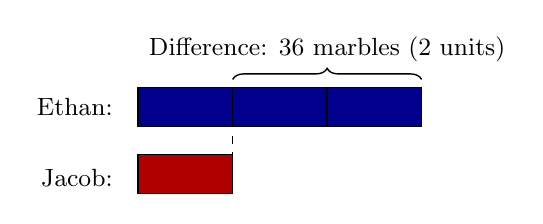
\begin{tikzpicture}[>=Stealth, baseline={(0,0.5)}]
    \node[anchor=east] at (-0.2, 0.9) {\small Ethan:};
    \draw[fill=bluebar, draw=black, line width=0.5pt] (0, 0.65) rectangle (3.6, 1.15);
    \foreach \x in {1.2, 2.4} { \draw[line width=0.5pt] (\x, 0.65) -- (\x, 1.15); }

    \node[anchor=east] at (-0.2, 0.0) {\small Jacob:};
    \draw[fill=redbar, draw=black, line width=0.5pt] (0, -0.2) rectangle (1.2, 0.3);

    \draw[dashed, line width=0.5pt] (1.2, -0.2) -- (1.2, 1.15);
    \draw[decorate, decoration={brace, amplitude=4pt}, line width=0.5pt] (1.2, 1.25) -- (3.6, 1.25);
    \node[anchor=south] at (2.4, 1.35) {\small Difference: 36 marbles (2 units)};
  \end{tikzpicture}

  \vspace{0.6em}
  2 units = 36 $\implies$ 1 unit = $\underline{\hspace{1.2cm}}$ \\
  Total units = $3 + 1 = 4$ units $\implies$ Altogether = $4 \times \underline{\hspace{1.2cm}} = \underline{\hspace{1.5cm}}$ marbles

\end{enumerate}

\clearpage

% ================= PART 3: REPEATED IDENTITY & SCALING =================
\section*{Part 3: Repeated Identity \& Scaling (Multiplication \& Division)}

\begin{enumerate}[label=\textbf{\arabic*.}, start=11, itemsep=2.5em, leftmargin=2em]

  \vspace{1em}
  % Question 11
  \item \textbf{A length of rope is divided into 6 equal parts. If 4 parts measure 48 cm, what is the total length of the rope?}

  \vspace{0.5em}
  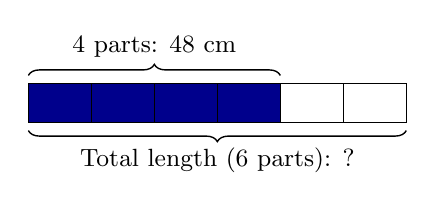
\begin{tikzpicture}[>=Stealth, baseline={(0,0.5)}]
    \draw[fill=bluebar, draw=black, line width=0.5pt] (0, 0.6) rectangle (3.2, 1.1);
    \draw[fill=white, draw=black, line width=0.5pt] (3.2, 0.6) rectangle (4.8, 1.1);
    \foreach \x in {0.8, 1.6, 2.4, 3.2, 4.0} { \draw[line width=0.5pt] (\x, 0.6) -- (\x, 1.1); }

    \draw[decorate, decoration={brace, amplitude=4pt}, line width=0.5pt] (0, 1.2) -- (3.2, 1.2);
    \node[anchor=south] at (1.6, 1.3) {\small 4 parts: 48 cm};

    \draw[decorate, decoration={brace, amplitude=4pt, mirror}, line width=0.5pt] (0, 0.5) -- (4.8, 0.5);
    \node[anchor=north] at (2.4, 0.4) {\small Total length (6 parts): ?};
  \end{tikzpicture}

  \vspace{0.6em}
  1 part = $48 \div 4 = \underline{\hspace{1.2cm}}$ cm
  \hspace{2cm} Total length = $6 \times \underline{\hspace{1.2cm}} = \underline{\hspace{1.5cm}}$ cm

  \vspace{1em}
  % Question 12
  \item \textbf{A tablet costs 5 times as much as a smartwatch. If the tablet costs \$640 more than the smartwatch, how much does the smartwatch cost?}

  \vspace{0.5em}
  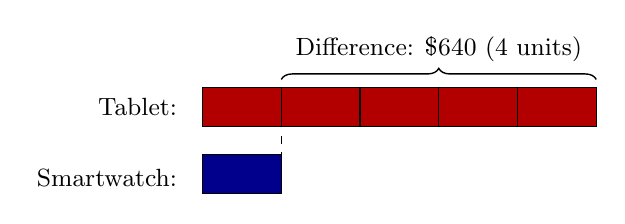
\begin{tikzpicture}[>=Stealth, baseline={(0,0.5)}]
    \node[anchor=east] at (-0.2, 0.9) {\small Tablet:};
    \draw[fill=redbar, draw=black, line width=0.5pt] (0, 0.65) rectangle (5.0, 1.15);
    \foreach \x in {1.0, 2.0, 3.0, 4.0} { \draw[line width=0.5pt] (\x, 0.65) -- (\x, 1.15); }

    \node[anchor=east] at (-0.2, 0.0) {\small Smartwatch:};
    \draw[fill=bluebar, draw=black, line width=0.5pt] (0, -0.2) rectangle (1.0, 0.3);

    \draw[dashed, line width=0.5pt] (1.0, -0.2) -- (1.0, 1.15);
    \draw[decorate, decoration={brace, amplitude=4pt}, line width=0.5pt] (1.0, 1.25) -- (5.0, 1.25);
    \node[anchor=south] at (3.0, 1.35) {\small Difference: \$640 (4 units)};
  \end{tikzpicture}

  \vspace{0.6em}
  4 units = \$640 $\implies$ 1 unit = $\$640 \div 4 = \underline{\hspace{1.5cm}}$ \\
  Smartwatch cost (1 unit) = \$\underline{\hspace{1.5cm}}

  \vspace{1em}
  % Question 13
  \item \textbf{Ryan and Sophie had \$180 in total. After Ryan spent \$30, he had 2 times as much money as Sophie. How much money did Ryan have initially?}

  \vspace{0.5em}
  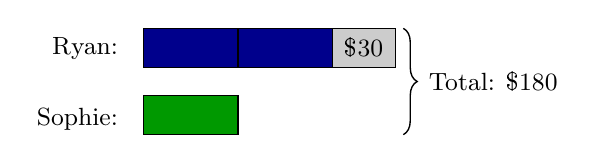
\begin{tikzpicture}[>=Stealth, baseline={(0,0.5)}]
    \node[anchor=east] at (-0.2, 0.9) {\small Ryan:};
    \draw[fill=bluebar, draw=black, line width=0.5pt] (0, 0.65) rectangle (2.4, 1.15);
    \draw[line width=0.5pt] (1.2, 0.65) -- (1.2, 1.15);
    \draw[fill=gray!40, draw=black, line width=0.5pt] (2.4, 0.65) rectangle (3.2, 1.15);
    \node at (2.8, 0.9) {\small\$\text{30}};

    \node[anchor=east] at (-0.2, 0.0) {\small Sophie:};
    \draw[fill=greenbar, draw=black, line width=0.5pt] (0, -0.2) rectangle (1.2, 0.3);

    \draw[decorate, decoration={brace, amplitude=5pt}, line width=0.5pt] (3.3, 1.15) -- (3.3, -0.2);
    \node[anchor=west] at (3.5, 0.475) {\small Total: \$180};
  \end{tikzpicture}

  \vspace{0.6em}
  Remaining total = $\$180 - \$30 = \underline{\hspace{1.5cm}}$ \\
  3 units = $\underline{\hspace{1.5cm}} \implies 1 \text{ unit} = \underline{\hspace{1.5cm}}$ \\
  Ryan initially = $2 \text{ units} + \$30 = 2 \times \underline{\hspace{1.2cm}} + 30 = \$\underline{\hspace{1.5cm}}$

  \vspace{1em}
  % Question 14
  \item \textbf{The total height of Tree A and Tree B is 150 cm. Tree A is $\frac{2}{3}$ the height of Tree B. Find the height of Tree B.}

  \vspace{0.5em}
  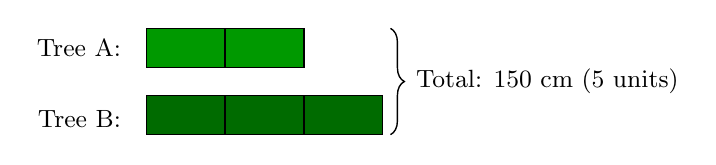
\begin{tikzpicture}[>=Stealth, baseline={(0,0.5)}]
    \node[anchor=east] at (-0.2, 0.9) {\small Tree A:};
    \draw[fill=greenbar, draw=black, line width=0.5pt] (0, 0.65) rectangle (2.0, 1.15);
    \draw[line width=0.5pt] (1.0, 0.65) -- (1.0, 1.15);

    \node[anchor=east] at (-0.2, 0.0) {\small Tree B:};
    \draw[fill=greenbar!70!black, draw=black, line width=0.5pt] (0, -0.2) rectangle (3.0, 0.3);
    \foreach \x in {1.0, 2.0} { \draw[line width=0.5pt] (\x, -0.2) -- (\x, 0.3); }

    \draw[decorate, decoration={brace, amplitude=5pt}, line width=0.5pt] (3.1, 1.15) -- (3.1, -0.2);
    \node[anchor=west] at (3.3, 0.475) {\small Total: 150 cm (5 units)};
  \end{tikzpicture}

  \vspace{0.6em}
  5 units = 150 cm $\implies$ 1 unit = $\underline{\hspace{1.2cm}}$ cm \\
  Height of Tree B (3 units) = $3 \times \underline{\hspace{1.2cm}} = \underline{\hspace{1.5cm}}$ cm

\end{enumerate}

\clearpage

% ================= PART 4: ADVANCED / MULTI-STEP PROBLEMS =================
\section*{Part 4: Advanced / Multi-Step Problems}

\begin{enumerate}[label=\textbf{\arabic*.}, start=15, itemsep=2.5em, leftmargin=2em]

  \vspace{1em}
  % Question 15

  \item \textbf{David had \$300. He spent
  $\frac{1}{3}$ of his money on books and $\frac{1}{4}$ of the remaining
  money on lunch. How much money did he have left?}

  \vspace{0.5em}

  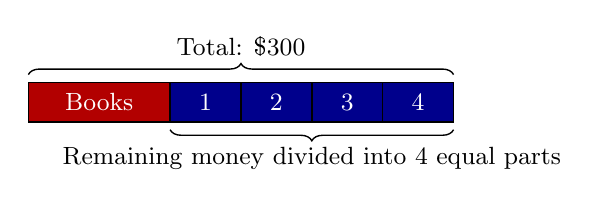
\begin{tikzpicture}[>=Stealth, baseline={(0,0.5)}]

    % Whole bar: 1/3 books + 2/3 remaining
    \draw[fill=redbar, draw=black, line width=0.5pt]
      (0, 0.6) rectangle (1.8, 1.1);

    \draw[fill=bluebar, draw=black, line width=0.5pt]
      (1.8, 0.6) rectangle (5.4, 1.1);

    % Divide the remaining 2/3 into 4 equal parts
    \foreach \x in {2.7, 3.6, 4.5} {
      \draw[line width=0.5pt] (\x, 0.6) -- (\x, 1.1);
    }

    % Labels
    \node at (0.9, 0.85) {\small\color{white}Books};

    \node at (2.25, 0.85) {\small\color{white}1};
    \node at (3.15, 0.85) {\small\color{white}2};
    \node at (4.05, 0.85) {\small\color{white}3};
    \node at (4.95, 0.85) {\small\color{white}4};

    % Whole bar
    \draw[decorate, decoration={brace, amplitude=4pt},
      line width=0.5pt]
      (0, 1.2) -- (5.4, 1.2);

    \node[anchor=south] at (2.7, 1.3) {\small Total: \$300};

    % Remaining section
    \draw[decorate, decoration={brace, amplitude=4pt, mirror},
      line width=0.5pt]
      (1.8, 0.5) -- (5.4, 0.5);

    \node[anchor=north] at (3.6, 0.4)
      {\small Remaining money divided into 4 equal parts};

  \end{tikzpicture}

  \vspace{0.6em}

  Money after books = \$300 - $\frac{1}{3}(300)$
  = \underline{\hspace{1.5cm}} \\

  Lunch cost = $\frac{1}{4} \times
  \underline{\hspace{1.5cm}}$
  = \underline{\hspace{1.5cm}} \\

  Money left = \underline{\hspace{1.5cm}}
  - \underline{\hspace{1.5cm}}
  = \$\underline{\hspace{1.5cm}}

  \vspace{1em}

  % Question 16
  \item \textbf{Alex had \$120 and Ben had \$45. After both received the same allowance amount from their parents, Alex had twice as much money as Ben. How much allowance did each receive?}

  \vspace{0.5em}
  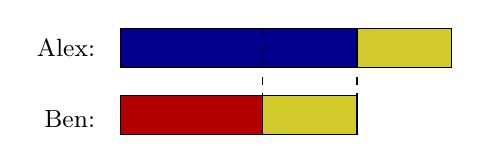
\begin{tikzpicture}[>=Stealth, baseline={(0,0.5)}]
    \node[anchor=east] at (-0.2, 0.9) {\small Alex:};
    \draw[fill=bluebar, draw=black, line width=0.5pt] (0, 0.65) rectangle (3.0, 1.15);
    \draw[fill=yellowbar, draw=black, line width=0.5pt] (3.0, 0.65) rectangle (4.2, 1.15);

    \node[anchor=east] at (-0.2, 0.0) {\small Ben:};
    \draw[fill=redbar, draw=black, line width=0.5pt] (0, -0.2) rectangle (1.8, 0.3);
    \draw[fill=yellowbar, draw=black, line width=0.5pt] (1.8, -0.2) rectangle (3.0, 0.3);

    \draw[dashed, line width=0.5pt] (1.8, -0.2) -- (1.8, 1.15);
    \draw[dashed, line width=0.5pt] (3.0, -0.2) -- (3.0, 1.15);
  \end{tikzpicture}

  \vspace{0.6em}
  Difference in money (unchanged) = $\$120 - \$45 = \$\underline{\hspace{1.5cm}}$ \\
  In the end, Alex has 2 units and Ben has 1 unit. Difference = $1 \text{ unit} = \$\underline{\hspace{1.5cm}}$ \\
  Ben's final amount = \$\underline{\hspace{1.5cm}} $\implies$ Allowance = $\underline{\hspace{1.5cm}} - 45 = \$\underline{\hspace{1.5cm}}$

  \vspace{1em}

  % Question 17
  \item \textbf{In a classroom, $\frac{3}{5}$ of the students were boys. After 6 boys left and 6 girls joined the class, $\frac{1}{2}$ of the students were boys. How many students were in the classroom altogether?}

  \vspace{0.5em}
  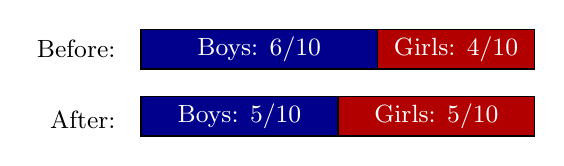
\begin{tikzpicture}[>=Stealth, baseline={(0,0.5)}]
    \node[anchor=east] at (-0.2, 0.9) {\small Before:};
    \draw[fill=bluebar, draw=black, line width=0.5pt] (0, 0.65) rectangle (3.0, 1.15);
    \draw[fill=redbar, draw=black, line width=0.5pt] (3.0, 0.65) rectangle (5.0, 1.15);
    \node at (1.5, 0.9) {\small\color{white}Boys: 6/10};
    \node at (4.0, 0.9) {\small\color{white}Girls: 4/10};

    \node[anchor=east] at (-0.2, 0.0) {\small After:};
    \draw[fill=bluebar, draw=black, line width=0.5pt] (0, -0.2) rectangle (2.5, 0.3);
    \draw[fill=redbar, draw=black, line width=0.5pt] (2.5, -0.2) rectangle (5.0, 0.3);
    \node at (1.25, 0.05) {\small\color{white}Boys: 5/10};
    \node at (3.75, 0.05) {\small\color{white}Girls: 5/10};
  \end{tikzpicture}

  \vspace{0.6em}
  Before fraction of boys = $\frac{3}{5} = \frac{6}{10}$. After fraction of boys = $\frac{1}{2} = \frac{5}{10}$. \\
  Change in boys = $\frac{6}{10} - \frac{5}{10} = \frac{1}{10}$ of total class. \\
  $\frac{1}{10}$ of class = 6 students $\implies$ Total students = $6 \times 10 = \underline{\hspace{1.5cm}}$

  \clearpage
  
  % Question 18
  \item \textbf{Container X has 45 liters of water and Container Y has 15 liters. How much water must be poured from Container X into Container Y so that both containers have equal volumes?}

  \vspace{0.5em}
  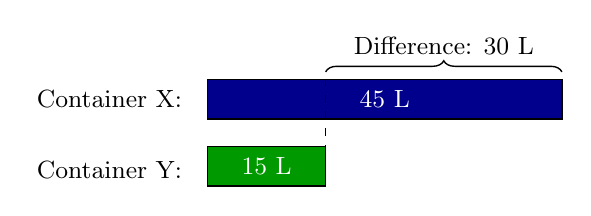
\begin{tikzpicture}[>=Stealth, baseline={(0,0.5)}]
    \node[anchor=east] at (-0.2, 0.9) {\small Container X:};
    \draw[fill=bluebar, draw=black, line width=0.5pt] (0, 0.65) rectangle (4.5, 1.15);
    \node at (2.25, 0.9) {\small\color{white}45 L};

    \node[anchor=east] at (-0.2, 0.0) {\small Container Y:};
    \draw[fill=greenbar, draw=black, line width=0.5pt] (0, -0.2) rectangle (1.5, 0.3);
    \node at (0.75, 0.05) {\small\color{white}15 L};

    \draw[dashed, line width=0.5pt] (1.5, -0.2) -- (1.5, 1.15);
    \draw[decorate, decoration={brace, amplitude=4pt}, line width=0.5pt] (1.5, 1.25) -- (4.5, 1.25);
    \node[anchor=south] at (3.0, 1.35) {\small Difference: 30 L};
  \end{tikzpicture}

  \vspace{0.6em}
  Difference = $45 - 15 = 30$ liters. \\
  Amount to transfer = $\text{Difference} \div 2 = 30 \div 2 = \underline{\hspace{1.5cm}}$ liters

  \vspace{1em}

  % Question 19
  \item \textbf{A basket of apples was shared among three children. The first child took $\frac{1}{2}$ of the apples plus 1 apple. The second child took $\frac{1}{2}$ of the remaining apples plus 1 apple. The third child received the remaining 4 apples. How many apples were in the basket at first?}

  \vspace{0.5em}
  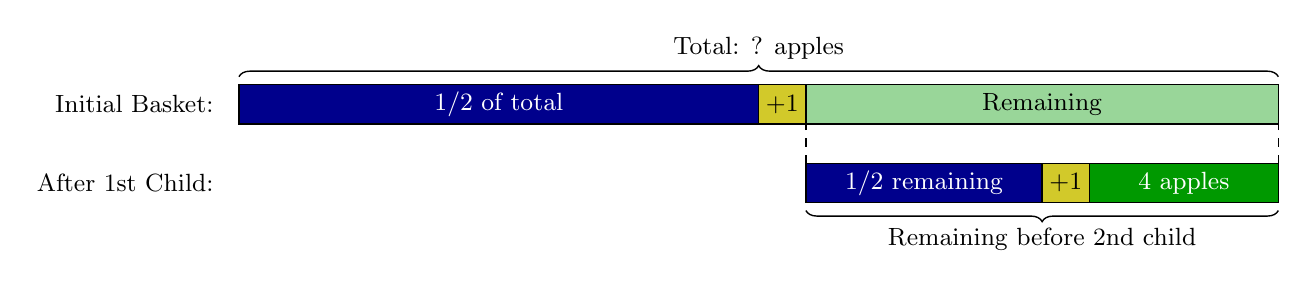
\begin{tikzpicture}[>=Stealth, baseline={(0,0.5)}]
    % --- Top Bar: Initial State (Scaled x2: Total = 44 blocks = 13.2 cm) ---
    \node[anchor=east] at (-0.2, 1.85) {\small Initial Basket:};
    
    % First child: 1/2 of total (22 blocks = 6.6 cm)
    \draw[fill=bluebar, draw=black, line width=0.5pt] (0, 1.6) rectangle (6.6, 2.1);
    \node at (3.3, 1.85) {\small\color{white}1/2 of total};

    % First child: +1 apple (2 blocks = 0.6 cm)
    \draw[fill=yellowbar, draw=black, line width=0.5pt] (6.6, 1.6) rectangle (7.2, 2.1);
    \node at (6.9, 1.85) {\small +1};

    % Remaining after 1st child (20 blocks = 6.0 cm)
    \draw[fill=greenbar!40, draw=black, line width=0.5pt] (7.2, 1.6) rectangle (13.2, 2.1);
    \node at (10.2, 1.85) {\small Remaining};

    % Top bracket: Total
    \draw[decorate, decoration={brace, amplitude=4pt}, line width=0.5pt] (0, 2.2) -- (13.2, 2.2);
    \node[anchor=south] at (6.6, 2.3) {\small Total: ? apples};

    % --- Bottom Bar: Remaining State (Scaled x2: Total = 20 blocks = 6.0 cm, aligned from 7.2 cm to 13.2 cm) ---
    \node[anchor=east] at (-0.2, 0.85) {\small After 1st Child:};

    % Second child: 1/2 of remaining (10 blocks = 3.0 cm)
    \draw[fill=bluebar, draw=black, line width=0.5pt] (7.2, 0.6) rectangle (10.2, 1.1);
    \node at (8.7, 0.85) {\small\color{white}1/2 remaining};

    % Second child: +1 apple (2 blocks = 0.6 cm)
    \draw[fill=yellowbar, draw=black, line width=0.5pt] (10.2, 0.6) rectangle (10.8, 1.1);
    \node at (10.5, 0.85) {\small +1};

    % Third child: 4 apples remaining (8 blocks = 2.4 cm)
    \draw[fill=greenbar, draw=black, line width=0.5pt] (10.8, 0.6) rectangle (13.2, 1.1);
    \node at (12.0, 0.85) {\small\color{white}4 apples};

    % Dashed alignment guide
    \draw[dashed, line width=0.5pt] (7.2, 1.1) -- (7.2, 1.6);
    \draw[dashed, line width=0.5pt] (13.2, 1.1) -- (13.2, 1.6);

    % Bottom bracket: Remaining before 2nd child
    \draw[decorate, decoration={brace, amplitude=4pt, mirror}, line width=0.5pt] (7.2, 0.5) -- (13.2, 0.5);
    \node[anchor=north] at (10.2, 0.4) {\small Remaining before 2nd child};
  \end{tikzpicture}
  
  \vspace{0.6em}
  Step 1 (Before 2nd child): $(4 + 1) \times 2 = \underline{\hspace{1.2cm}}$ apples \\
  Step 2 (Before 1st child / Total): $(\underline{\hspace{1.2cm}} + 1) \times 2 = \underline{\hspace{1.5cm}}$ apples
  
  \vspace{1em}

  % Question 20
  \item \textbf{A pencil and an eraser together cost \$2.40. Two pencils and three erasers together cost \$5.70. What is the cost of one pencil?}

  \vspace{0.5em}
  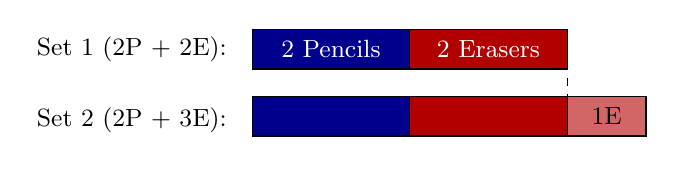
\begin{tikzpicture}[>=Stealth, baseline={(0,0.5)}]
    \node[anchor=east] at (-0.2, 0.9) {\small Set 1 (2P + 2E):};
    \draw[fill=bluebar, draw=black, line width=0.5pt] (0, 0.65) rectangle (2.0, 1.15);
    \draw[fill=redbar, draw=black, line width=0.5pt] (2.0, 0.65) rectangle (4.0, 1.15);
    \node at (1.0, 0.9) {\small\color{white}2 Pencils};
    \node at (3.0, 0.9) {\small\color{white}2 Erasers};

    \node[anchor=east] at (-0.2, 0.0) {\small Set 2 (2P + 3E):};
    \draw[fill=bluebar, draw=black, line width=0.5pt] (0, -0.2) rectangle (2.0, 0.3);
    \draw[fill=redbar, draw=black, line width=0.5pt] (2.0, -0.2) rectangle (4.0, 0.3);
    \draw[fill=redbar!60, draw=black, line width=0.5pt] (4.0, -0.2) rectangle (5.0, 0.3);
    \node at (4.5, 0.05) {\small 1E};

    \draw[dashed, line width=0.5pt] (4.0, -0.2) -- (4.0, 1.15);
  \end{tikzpicture}

  \vspace{0.6em}
  Cost of 2 pencils + 2 erasers = $2 \times \$2.40 = \$\underline{\hspace{1.5cm}}$ \\
  Cost of 1 eraser = $\$5.70 - \$\underline{\hspace{1.5cm}} = \$\underline{\hspace{1.5cm}}$ \\
  Cost of 1 pencil = $\$2.40 - \$\underline{\hspace{1.5cm}} = \$\underline{\hspace{1.5cm}}$

\end{enumerate}

\end{document}